\documentclass[a4paper,12pt]{article}
\parindent 0pt
\parskip 1mm
\usepackage{amsmath}
\usepackage[dvips]{epsfig}

\begin{document}

\begin{center}

{\Large\bf CN 510 - Principles and Methods of Cognitive and Neural Modeling}

\bigskip

{\large\bf Assignment \# 10}
\smallskip

{\large\bf John Joseph}
\end{center}

\bigskip
{\bf Pair-Based STDP and Correlated Input}
\bigskip

For our final assignment we are bringing together the work from Assignments 6 and 8 in which we dealt with the notion of plasticity. We generate a pre-synaptic network of 100 neurons with a correlated series of inputs that are passed on to a post-synaptic network of 20 neurons. The presence of these inputs will cause our post-synaptic neurons to fire, and by examining the temporal attributes of these post-synaptic potentials we derive the notion of plasticity. 

\vspace{2mm}

Our learning model is based loosely on the Hebbian theory stating that bond strength between neurons grows when the two fire within close temporal proximity of one another. Furthemore, these firings must maintain temporal causality; that is, the pre-synaptic neuron must fire before the post-synaptic neuron. 

\vspace{2mm}

Our learning rule, called the additive rule, is as follows: at some time %t=n$,

\begin{equation}
\Delta w_{ij}(n) = \eta (S_j(n)x_{i}(n)-S_i(n)x_j(n))
\end{equation}

Where the indices $i$ and $j$ represent our pre-synaptic and post-synaptic neurons, respectively and $S$ represents the presence (or absence) of a spike. $\eta$ is a learning rate, which was set in the handout as 0.02. I often found that this value had to be changed; one would assume this could be related to my units of time, which were milliseconds, but I ended up using $\nu=0.2$. This is neither 1000x nor 0.001x the original number, so I can't explain this very well. 

\vspace{2mm}

However, my motivations were to generate good looking results, and in this regard I actually did suprisingly OK. The previous assignments dealing with plasticity were huge problems for me, and I never got my network to exhibit anything close to plasticity. However, I managed to find a number of bugs in the code from those assignments, and now that they are fixed I'm starting to see much more plausible results. 

\vspace{2mm}

Things still are not perfect, and I'd like to spend some time to focus on my units of both time and voltage. However, in terms of network dynamics I think my figures will show that the bonds within my network were in fact modified based on the learning rule outlined above. 


\bigskip
{\bf Results}
\bigskip

First of all, sorry about placing my figures at the very end. LaTex was not playing nice. 

\vspace{2mm} 

To generate my results for the pre-synaptic and post-synaptic traces I went through a bit of a trial and error process. What I mean is, though there were 100*20=2000 bonds in my network, I was not willing to output all of these into text files to sort through in gnuplot. 

\vspace{2mm}

Given that my results were random, I output the first 10 bonds and essentially ran the network till I got something interesting. My plots show the bond between two neurons and the bond strength between them; this bond strength is merely the weight I assigned to the bond, and in my graphs you can see how this weight changed with time. 

\vspace{2mm}

I tried to show examples where the bonds were both strengthened and weakened, as the rule accomodates for both. We weaken the bond in the case where a pre-synaptic spike occurs after a post-synaptic spike, which seems to be an inhibitory rule more than anything else. The weights were also clamped between 0 and 1 to prevent any instabilities from occuring; without this check I had seen values go as high as $10^{36}$. For the record, these learning and unlearning examples are from two different neurons and show both of their evolutions through time; I apologize for not giving a zoomed out version of the unlearning, but it was nothing fascinating. 

\vspace{2mm}

The two histograms show the weight distribution of my network before and after the simulation; the initial weights were distributed randomly using a psuedorandom number generator, but the final weights have clearly settled down. One thing to note is that in the lecture we had been told the Additive rule, which is the learning rule I used, should generate an ``all or nothing'' network in which one bond dominates over the rest (I think). This was not the case, as there were a good number of neurons in my network with values between 0 and 1. 

\vspace{2mm}

However, a the majority of neurons did converge to 0 by the end of the simulation, and of the nonzero bonds the ones with maximum strength were the most prevalent. This could arguably be considered a bimodal distribution; there are two statistical modes at 1 and 0, though the intermediary values do bother me.  

{\bf Other Rules and Further Discussion}

For the sake of curiosity I tried to implement the power  and multiplicative learning rules outlined in the paper by Morrison et. al. Below are the weight distributions for these two rules; we see a roughly unimodal distribution for the multiplicative rule.

\vspace{2mm}

For the power rule, I plotted two different values of $\mu$:0.02 and 0.8. The paper states that a value of 0 and 1 should correspond to the additive and multiplicative rules, respectively. Thus we expect to see bimodal distributions for lower values of $\mu$ and unimodal distributions for the higher values, and this is exactly what we produce. My code for doing this is as follows:

\begin{verbatim}
for (i=0;i<100;i++)
  for (j=0;j<20;j++)
    dW[20*i+j] = nu*
      (pow((wMax-pre[i].w[j]),mu)*pre[i].x*post[j].s-
      pow(pre[i].w[j],mu)*post[j].x*pre[i].s);
\end{verbatim}

While this does satisfy the requirements for extra credit, it feels a little cheap. I have no clue how to derive the critical $\mu$ value, but I knew what very low and very high values ought to do based on the formulas. As such I picked a very low and very high value and saw what I expected to see. I apologize for not making the bar graphs solid red; it's literally 10:53 am and I am going to class now. This was a fun assignment, and I'm glad I got results that made sense. 

\vfil\eject

\begin{center}
  \begin{figure}[h!]
    \epsfig{file=data/initialHistogram,width=13cm,height=8cm}
    \caption{\label{pict1}Initial Histogram with Random Distribution}
  \end{figure}
\end{center}

\begin{center}
  \begin{figure}[h!]
    \epsfig{file=data/finalHistogram,width=13cm,height=8cm}
    \caption{\label{pict1}Final Histogram of Weight Distribution}
  \end{figure}
\end{center}

\begin{center}
  \begin{figure}[h!]
    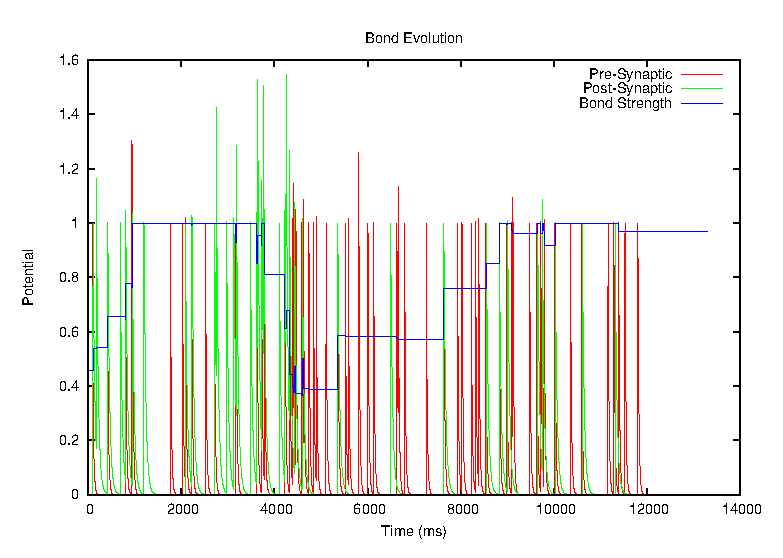
\epsfig{file=data/causality4,width=13cm,height=8cm}
    \caption{\label{pict1}The bond evolution of two neurons and their traces}
  \end{figure}
\end{center}

\begin{center}
  \begin{figure}[h!]
    \epsfig{file=data/causality4_Zoom,width=13cm,height=8cm}
    \caption{\label{pict1}A zoom on the bond evolution; note the causality-induced learning}
  \end{figure}
\end{center}

\begin{center}
  \begin{figure}[h!]
    \epsfig{file=data/causality4_unlearn,width=13cm,height=8cm}
    \caption{\label{pict1}An example of unlearning, wherein two pre-synaptic spikes fall within a post-synaptic decay, exhibiting the same temporal causality}
  \end{figure}
\end{center}

\begin{center}
  \begin{figure}[h!]
    \epsfig{file=data/multDist,width=13cm,height=8cm}
    \caption{\label{pict1}The multiplicative rule leads to a unimodal distribution}
  \end{figure}
\end{center}

\begin{center}
  \begin{figure}[h!]
    \epsfig{file=data/powerDistlow,width=13cm,height=8cm}
    \caption{\label{pict1}The power rule with lower values leads to a bimodal distribution of weights}
  \end{figure}
\end{center}

\begin{center}
  \begin{figure}[h!]
    \epsfig{file=data/powerDisthigh,width=13cm,height=8cm}
    \caption{\label{pict1}The power rule with higher $\mu$ values leads to a unimodal distribution of weights}
  \end{figure}
\end{center}

\end{document}
